%% Versão final IEEE
\documentclass[a4paper]{IEEEtran}

% Versão 
%\documentclass[journal,12pt,onecolumn,draftclsnofoot,]{IEEEtran}
%\usepackage[a4paper, marginparwidth=1in]{geometry}




\usepackage[utf8]{inputenc}
\usepackage{epstopdf}
%\usepackage[spanish]{babel}
\usepackage[cmex10]{amsmath}
%\interdisplaylinepenalty=2500
\usepackage{amsfonts}
\usepackage{amssymb}
\usepackage{graphicx}
\usepackage{verbatim}
\usepackage{array}
\usepackage{multirow}
\usepackage{dcolumn}
\usepackage{color}
\usepackage[noadjust]{cite}
\usepackage{url}
\usepackage{balance}
\usepackage[usenames,dvipsnames]{xcolor}
\usepackage{accents}
\usepackage{blindtext}
%\usepackage{soul}
\usepackage[normalem]{ulem}
%\DeclareGraphicsExtensions{.eps} % eu que comentei
%\AppendGraphicsExtensions{.pdf} % eu que comentei


% % % Adicionados por mim
%\usepackage[colorinlistoftodos]{todonotes}
\usepackage[colorinlistoftodos,prependcaption,textsize=tiny]{todonotes}
\usepackage{xargs} 

\newcommandx{\todoi}[2][1=]{\todo[linecolor=Plum,backgroundcolor=Plum!25,bordercolor=Plum,#1,inline]{#2}}
%\newcommand{\todop}[1]{\todo[textsize=tiny]{#1}}
%%%%



\DeclareMathOperator*{\Max}{max}
\DeclareMathOperator*{\Min}{min}
\DeclareMathOperator*{\argmin}{arg\,min}
\DeclareMathOperator*{\Maximize}{Maximize}

\begin{document}
\title{Nongaussian time series model via Quantile Regression}

\author{Marcelo~Ruas,~\IEEEmembership{Student Member,~IEEE,}
	    and Alexandre~Street,~\IEEEmembership{Member,~IEEE}	


%\thanks{This work was partially supported by UTE Parna\'iba Gera\c{c}\~ao de Energia S.A. through R\&D project ANEEL PD-7625-0001/2013.}
%\thanks{Bruno Fanzeres, Arthur Brigatto and Alexandre Street are with the Electrical Engineering Department, Pontifical Catholic University of Rio de Janeiro (PUC-Rio), Rio de Janeiro, RJ, Brazil (e-mail: \mbox{bsantos@ele.puc-rio.br}; \mbox{street@ele.puc-rio.br}).}
%\thanks{L. A. Barroso are with PSR Consulting, Rio de Janeiro, RJ, Brazil (e-mail: \mbox{luiz@psr-inc.com}).}
}

\maketitle


\begin{abstract}
	\blindtext
\end{abstract}

\begin{IEEEkeywords}
	Quantile Regression, Model Identification, Non-gaussian time series model
\end{IEEEkeywords}


\listoftodos


% ===== Sec. I - Introduction ===== %

\section{Introduction}

% % % Talk about renewable energy and its variability

Renewable energy power is a hot topic in the recent years. It is a much cleaner way of producing energy than by using other sources such as coal and gas, and with less hazard potential than nuclear power plants. The installed capacity of renewable plants has been increasing in a fast pace and projections point that wind power alone will account to 18\% of global power by 2050  \cite{IntEnerAgency}.
In spite of being a welcoming technology, it brings new challenges for power system planners, operators, and agents. It is important to have good forecasts of either high and low quantiles
 the complex behavior of wind is very difficult to model and predict.  \todo{é importante prever bem quantis altos e baixos p analise de risco - fica prejudicada pela dificuldade de previsao destes quantis }
Having better prediction models can help the planner to make better and less risky decisions, increasing the attractiveness of renewable energy to the energy system. 
In this work we will investigate how to model dynamics of renewable energy time series in both short and long terms.

% % % Critics about point forecasts and gaussian models (ARIMA-GARCH). Compare GAS and nonparametric models. 

Conventional statistics are often focused on estimating the conditional mean of a given random variable.
\todoi{Falar sobre modelos de previsão usando modelos tradicionais para energia renovável}
 This is not very useful when dealing with renewable energy, as the variability and the notion of risk is extremely important for planning. Our attention is, then, turned to probabilistic forecasting models. Among these, there are many possibilities. \cite{zhang_review_2014} reviews the commonly used methodologies for this task, separating them in parametric and nonparametric classes. Main characteristics of \textbf{parametric models} are (i) assuming a distribution shape and (ii) low computational costs. ARIMA-GARCH, for example, model the renewable series by assuming the distribution \textit{a priori}. On the other hand, \textbf{nonparametric models} (i) don't require a distribution to be specified, (ii) needs mode data to produce a good approximation and (iii) have a higher computational cost. Popular methods are Quantile Regression, Kernel Density Estimation,  Artificial Intelligence or a mix of them.


% % % Talk about nonparametric models and how to use quantile regression to estimate the whole distribution

A common finding is that wind and solar time series don't have a Gaussian behavior. Furthermore, we can't point any distribution that fits on the data undoubtedly. For this reason, we choose to use a nonparametric approach, more specifically the Quantile Regression (QR), as defined in \cite{koenker2005quantile}.
As we are working with time series, we rely on the results of \cite{koenker_quantile_2006}, which defines the quantile autoregression, extending the application of QR on cases where the covariates are lagged values of $y_t$. 
QR is a powerful tool for measuring quantile others than the median. By estimating many quantiles on a thin grid of probabilities, one can have as many points as desired of the estimated conditional distribution function.

However, when estimating a distribution function, as each quantile is estimated independently, the monotonicity of the distribution function may be violated. This issue is a known as crossing-quantiles. To get around it we propose to either add a constraint on the optimization model or make a transformation as in \cite{chernozhukov_quantile_2010}, which can be estimated independently.

Using QR as in \cite{koenker2005quantile} is not a novelty when predicting the conditional distribution of wind power time series, as is already done in \cite{moller_time-adaptive_2008,nielsen2006,bremnes_probabilistic_2004,wan_direct_2017}.
In this article, we combine QR with regularization techniques. On the Mixed Integer Linear Programming (MILP) approach, we use the best subset selection, which \cite{bertsimas_best_2015} does for minimizing the quadratic error and the $\ell_1$ penalization as in \cite{belloni_l1-penalized_2009} or \cite{ciuperca_adaptive_2016} (the AdaLasso variant, where each coefficient may have a different weight on the objective function to ensure oracle properties).
On the advantages of QR we highlight the fact that it is a direct way of finding a given quantile directly and it is data driven, so it doesn't depend on distribution assumptions. 

%% Review of quantile regression for wind and solar

\todoi{Review of quantile regression for wind and solar - procurar mais referências?}

The approach by \cite{gallego2016line} is to use QR with a nonparametric methodology. The authors add a penalty term based on the Reproducing Kernel Hilbert Space, which allows a nonlinear relationship between the explanatory variables and the output. This paper also develops an on-line learning technique, where the model is easily updated after a new observation.

In \cite{wan_direct_2017}, QR is used with a special type of Neural Network (NN) with one hidden layer, called extreme learning machine. In this setup, each quantile is a different linear combination of the features of the hidden layer. 


 



%%%% Contributions
The objective of this paper is to propose a new methodology to address nonparametric time-series focused on renewable energy. In our analysis, we develop both nonlinear and linear models for QR. The main contributions are:
\begin{itemize}
	\item A nonparametric methodology to model the conditional distribution of a given time series.
	
	\item On the linear case, we propose a parsimonious methodology that selects the global optimal solution with a given number of 
	
	\item Regularization techniques applied to an ensemble of quantile regressions to estimate the conditional distribution
	
	\item 
	
\end{itemize}

We propose a new combination of methods to predict the $k$-step ahead conditional distribution. By using MILP, we achieve a solution which is optimal for the given objective. In order to improve the quality of predictions and interpretability, we incorporate a joint regularization by specifying the existence of groups among the probabilities $\alpha$. We could not find any other work in the literature that interpreted different quantiles as models depending on one another. 
The objective of this paper is to propose and test different techniques of predicting the conditional distribution based on QR. 


% OBJETIVOS:
Um modelo para séries tmeporais autoregressivo e nao parametrico e baseado na função quantilica. No caso autoregressivo, uma metodologia de estimação com seleção parcimoniosa otima global é proposta e possibilita o controle dos números de grupos de regressores diferentes dentro do modelo para diferentes quantis. Para o modelo não paramétrico
Modelo data driven, empirico


% Next sessions paragraph

The remaining of the paper is organized as follows. In section II, we present both the linear parametric and the nonlinear QR based time series models. In section III, we discuss the estimation procedures for them. The regularization strategies are also presented on this section. Finally, in section IV, a case study using real data from both solar and wind power is presented in order to ...
Section V will conclude this article.



%2) Quantile Regression based time series model
%	A. Linear parametric explanatory model
%	B. General non-linear nonparametric model
%
%3) Estimation procedures
%	A. Linear model with optimal variable selection / regularization
%	B. Nonlinear model
%	
%4) Case study
%	A. Long term wind power generation
%	B. Short term wind (solar?) generation
%
%5) Conclusion





% % Seguir a estrutura paragrafo papaer henrique

%1) Motivacao para minimizar o risco da WPG
%2) Fala sobre a pesquisa em WPG utilizando ARMA e SARIMA com distribuição gaussiana 

% % Colocar em especifico os objetivos e detalhar os papers anteriores, destacando o que o nosso tem e nenhum outro atingiu ate entao

% procurar os objetivos que já discutimos.









% % % % % % % % % % % % % % % % % % %

%As opposed to the conventional work of doing a model to forecast the
%conditional mean, our work focus on finding a distribution for $y_{t}$
%on each $t$. 
%
%We find a time series model, based on quantile autoregression (as
%in Koenker 2005).
%
%As we are interested in the whole distribution of $\hat{y}_{t+k|t}$,
%we estimate a phin grid of quantiles in $0<\alpha_{1}<\alpha_{2}<\dots<\alpha_{|A|}<1$,
%such that the distribution can be well approximated.
%
%As a Quantile Autoregression model, we are interested in selecting
%the best subset of variables do model the time series. 
%
%As we are trying to model the whole $k$-step ahead distribution,
%we estimate many quantiles. We didn't find any previous work where
%a given $\alpha$-quantile model influenced another model.
%
%In all works found, each quantile is estimated separately. 
%
%Regularization can be done by introducing a penalty on the $\ell_1$-norm of the coefficients. The work by \cite{belloni_l1-penalized_2009} defines proprieties and convergence analysis. The AdaLasso variant, where each coefficient may have a different weight on the objective function to ensure oracle proprieties, is developed on \cite{ciuperca_adaptive_2016}.

% ===== Sec. II - Quantile Regression ===== %

\section{Quantile Regression based time series model} \label{sec:qr1}

Let the $\alpha$-conditional quantile function of $Y$ for a given value $x$ of the $d$-dimensional random variable $X$, i.e., $Q_{Y|X}:[0,1] \times \mathbb{R}^d \rightarrow \mathbb{R}$, can be defined as %(in short, from now on, $Q_{Y|X}(\cdot, \cdot)$)
\begin{equation}
Q_{Y|X}(\alpha,x) = F_{Y|X}^{-1}(\alpha,x) = \inf\{y: F_{Y|X}(y,x) \geq \alpha\}.
\label{eq:quantile-function}
\end{equation}
Let a dataset be composed from $\{y_t,x_t \}_{t \in T}$ and let $\rho$ be the check function 
\begin{equation}\label{eq:check-function}
\rho_{\alpha}(x)=\begin{cases}
\alpha x & \text{if }x\geq0\\
(1-\alpha)x & \text{if }x<0
\end{cases}.
\end{equation}
The sample quantile function for a given probability $\alpha$ is then based on a finite number of observations and is the solution to minimizing the loss function $L(\cdot)$:
\begin{IEEEeqnarray}{C}
\hat{Q}_{Y|X}(\alpha,\cdot)\quad\in\quad  \underset{q\in\mathcal{Q}}{\text{arg min}}\, L_\alpha(q) = \sum_{t\in T}\rho_{\alpha}(y_{t}-q(x_t)),\label{eq:optim-lqr1} 
\end{IEEEeqnarray}
The $\alpha$-quantile function $q_\alpha$ belongs to a function space $\mathcal{Q}$. We might have different assumptions for space $\mathcal{Q}$, depending on the type of function we want to find for $q$. A few properties, however, must be achieved by our choice of space, such as being continuous and having limited first derivative. In this paper, we consider the case where $\mathcal{Q}$ is a linear function's space.

The quantile function is approximated by a sequence of $|J|$ (where $J$ is an index set) quantiles $q_{\alpha_1} \leq q_{\alpha_2} \leq \dots \leq q_{\alpha_{|J|}}$. 
We also define the closely related set $A = \{ \alpha_j \mid j \in J \}$, whose elements all must range on $[0,1]$, for they are probability values such that $0 < \alpha_1 < \alpha_2 < \dots < \alpha_{|J|} < 1$. The sequence $\{ \alpha_j \}_{j \in J}$ provides a finite discretization of the interval $[0,1]$. 

Problem (\ref{eq:optim-lqr1}) can be rewritten as a Linear Programming problem as in (\ref{eq:linear-opt-1})-(\ref{eq:linear-opt-ult}), thus being able to use a modern solver to fit our model. Variables $\varepsilon^+_t$ and $\varepsilon^-_t$ represent the quantities $|y-q(\cdot)|^+$ and $|y-q(\cdot)|^-$, respectively. This new formulation estimates all quantiles at the same time, and we denote $q$ as $q_\alpha$ to differentiate it from each $\alpha$.
{\tiny }\begin{IEEEeqnarray}{lr}
\min_{\beta_{0j},\beta_j,\varepsilon_{tj}^{+}, \varepsilon_{tj}^{-}} \, \sum_{j \in J} \sum_{t \in T}\left(\alpha_j \varepsilon_{t j}^{+}+(1-\alpha_j)\varepsilon_{t j}^{-}\right)
 \span \label{eq:linear-opt-1}\\
\mbox{subject to} \span \nonumber \\
\varepsilon_{t j}^{+}-\varepsilon_{t j}^{-}=y_{t} - \beta_{0j} - \beta_{j}^T x_{t}, & \forall t \in T, \forall j \in J, \\
\varepsilon_{tj}^+,\varepsilon_{tj}^- \geq 0, & \forall t \in T,\forall j \in J,\\ 
\beta_{0j} + \beta_{j}^T x_{t} \leq \beta_{0,j+1} + \beta_{j+1}^T x_{t}, \span \nonumber \\
\span \label{eq:linear-opt-ult} \forall t \in T, \forall j \in J_{(-1)},
\end{IEEEeqnarray}
To estimate a conditional distribution based on quantile values, all quantiles $\{q_\alpha \}_{\alpha \in A}$ are estimated simultaneously. With the addition of constraint (\ref{eq:linear-opt-ult}), we assure the monotonicity of the quantile function, solving the issue of crossing-quantiles.
The output is the sequence $\{ q_\alpha \}_{\alpha \in A}$, which is fully defined by the optimum values $\beta^*_{0\alpha}$ and $\beta^*_\alpha$, for each $\alpha$.

We apply QR to estimate the conditional distribution $\hat{Q}_{Y_{t+h}|X_{t+h},Y_t, Y_{t-1}, \dots} (\alpha,\cdot)$ for a $h$-step ahead forecast of time serie $\{y_t\}$, where $X_{t+h}$ is a vector of exogenous variables at the time we want to forecast. Once the conditional distribution is estimated, we are able to simulate and generate scenarios. In the next session, regularization techniques are presented, in order to choose parsimoniously which variables will be input for $\hat{Q}$.

%Let $A$ be a set containing a sequence of probabilities  $\alpha_i$ such that $0 < \alpha_1 < \alpha_2 < \dots < \alpha_Q < 1$. This set represents a finite discretization of the interval $[0,1]$.
%One of our goals with quantile regression is to estimate a quantile function $\hat{Q}_{Y|X}$ of a given real valued random variable $X$ from a sequence of quantiles $q_{\alpha_1}(x_t) \leq q_{\alpha_2}(x_t) \leq \dots \leq q_{\alpha_{|A|}}(x_t)$, with $0 < \alpha_1 < \alpha_2 < \dots < \alpha_{|A|} < 1$, for any given $t$.
%The process of fitting $\hat{Q}_{Y|X}$ is by mapping every $\alpha_i$ with its estimated quantile $\hat{q}_{\alpha_i}(x_t)$.
%The denser the grid of values in $A$, better is the approximation of $Q_{Y|X}$.
%Thus, the distribution found for $Y$ is nonparametric, as no previous assumptions are made about its shape, and its form is fully recovered by the data we have.
%
%The crossing quantile is a common issue when estimating a set of quantiles \cite{chernozhukov_quantile_2010}. Two a solution may be 
%
%
%A typical problem, however, arises when working with quantile regression. When quantiles are estimated independently, it is possible to find $q_{\alpha}(x_t) > q_{\alpha'}(x_t)$, for a given $t$, when $\alpha_1 < \alpha_2$. An example can be seen on Figure \ref{fig:crossing-quantiles}, where quantiles $\alpha = 0.95$ and $\alpha = 0.9$ cross. This problem, called \textit{crossing quantiles}, can be prevented by estimating all quantiles with a single minimization problem.
%
%
%
%As opposed to traditional parametric models where one has to assume the error distribution on the model
%\begin{equation}
%y_t = h(F_t) + \varepsilon_t,
%\end{equation}
%as we choose the nonparametric methodology we are released from this step. A distribution for $\varepsilon_t$ is defined within the estimation procedure. The predictive distribution is derived from the individual quantiles
%\begin{equation}
%\hat q^\alpha_{t+k|k} = \hat y_{t+k|t} + \hat F^\varepsilon_{t,k}(\alpha).
%\end{equation}
%% % coisas aqui % %
%\cite{wan_direct_2017} defines a model based on extreme machine learning to estimate every $\alpha$-quantile in a thin grid $0 < \alpha_1 < \alpha_2 < \dots < \alpha_Q < 1$. 
%	
%	
%	
%	
%	
%	
%%\subsection{Linear parametric explanatory model}
%%	\blindtext
%
%One of the options is to consider function $q_\alpha(\cdot)$ in problem (\ref{eq:optim-qr1})-(\ref{eq:optim-qr2}) as a linear function of its parameters. In this setup, 
%\begin{equation}
%\hat q_\alpha(x_t) = \beta^T x_t + \beta_0.
%\end{equation}
%
%\section{Regularization}
%Our study also (...) the regularization process together with the estimation of the conditional distribution function, which is a contribution in this paper.
%
%We investigate two ways of regularization.
%The first of them consists of selecting the best subset of variables through Mixed Integer Programming, given that $K$ variables are included in the model. 
%
%The second way is including a $\ell_1$ penalty on the linear quantile regression, 
%Both of them will be built over the standard Quantile Linear Regression model. In the end of the section, we discuss a information criteria to be used for quantile regression and verify how close are the solutions in the eyes of this criteria.
%
%When we choose $q_\alpha(x_t)$ to be a linear function
%\begin{equation}
%\hat{q}_\alpha(x_t) = \beta_{0\alpha} + \beta_\alpha^T x_t 
%\end{equation}
%we can substitute it on problem \ref{eq:qar-general}, getting the following LP problem:

	
	
%To model \ref{eq:linear-model} as a Linear Programming problem, thus being able to use a modern solver to fit our model,  we create variables $\varepsilon^+_t$ e $\varepsilon^-_t$ to represent the positive and the negative values of \ref{eq:check-function}, respectively. The optimal argument $q_\alpha^*(\cdot)$ on the Linear Programming problem \ref{eq:qar-general} is the estimated $\alpha$-quantile for the given random sample.
%\begin{equation}
%\begin{aligned}q^*_\alpha(.) \in \underset{q_\alpha (\cdot),\varepsilon_{t}^{+}, \varepsilon_{t}^{-}}{\text{arg min}} & \sum_{t \in T}\left(\alpha \varepsilon_{t}^{+}+(1-\alpha)\varepsilon_{t}^{-}\right) & \\
%\mbox{s.t. } & \varepsilon_{t}^{+}-\varepsilon_{t}^{-}=y_{t}-q_\alpha(x_t), & \qquad\forall t \in T,\\
%& \varepsilon_t^+,\varepsilon_t^- \geq 0, & \qquad \forall t \in T.
%\end{aligned}
%\label{eq:qar-general}
%\end{equation}
%
%	
%\subsection{General non-linear nonparametric model}
%	\blindtext
%	
%A quantile of a random variable is important in risk measuring, as we can measure the probability of occurrence of extreme events, and in many other fields. While working with energy forecasts, quantile regression can produce interesting results when working with both short term (hourly) or long term (monthly) data. As an example, we present a solar time series for the short term and a wind time series for long term. The first set of data is measured at the location of Tubarao (Brazil) on the year of 2014, while the latter is a dataset of mean power  monthly observations from Icaraizinho (Brazil) between 1981 to 2011 of measured in Megawatts. Figure \ref{fig:boxplots} illustrate the seasonality present in these datasets.
%
%\begin{figure}
%	\centering
%	\begin{minipage}[t]{\linewidth}
%		
%		\begin{minipage}[t]{0.45\linewidth}
%			%\centering
%			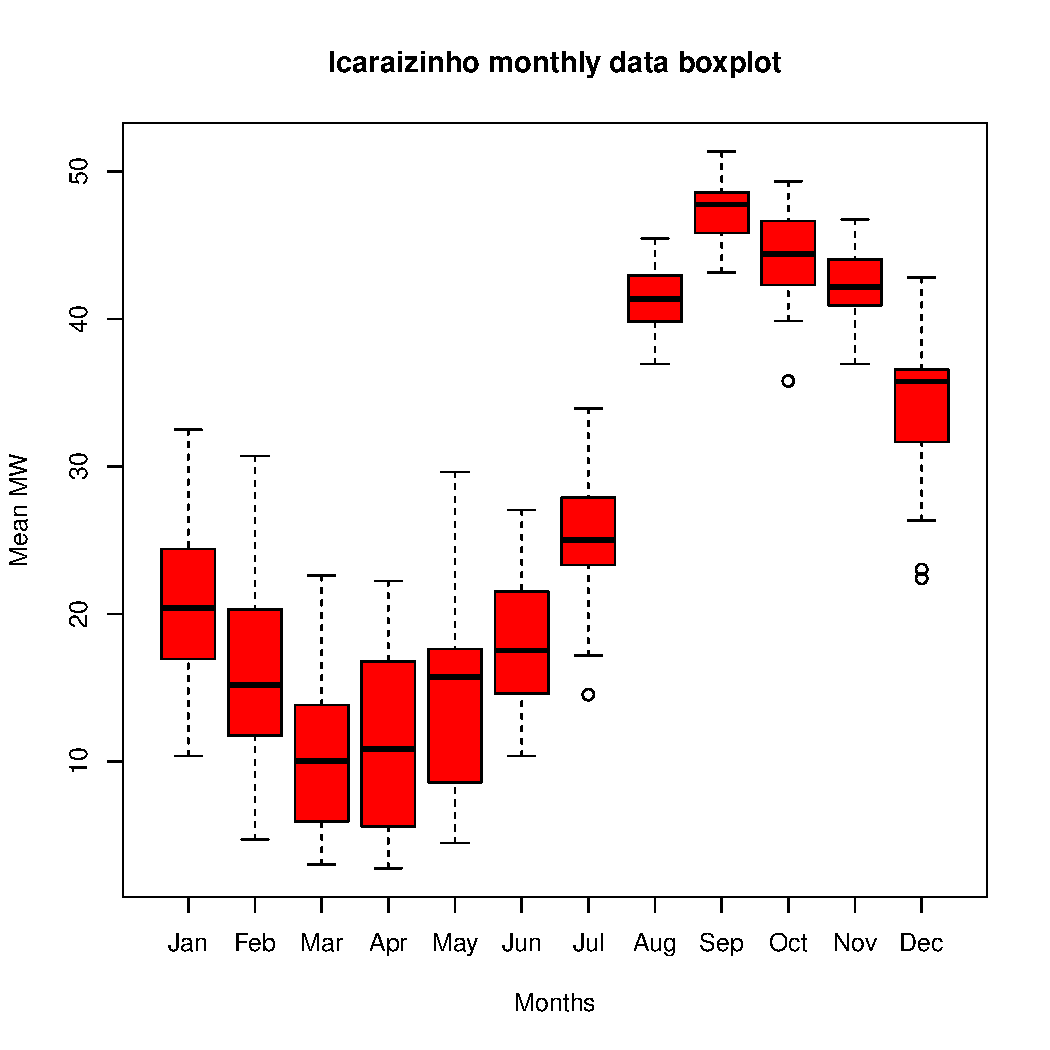
\includegraphics[width=\textwidth]{./../Figuras/Icaraizinho/icaraizinho-boxplot}
%			%\caption{Boxplot for each month for the Icaraizinho dataset}
%			\label{fig:icaraizinho-boxplot}
%		\end{minipage}
%		\begin{minipage}[t]{0.45\linewidth}
%			%\centering
%			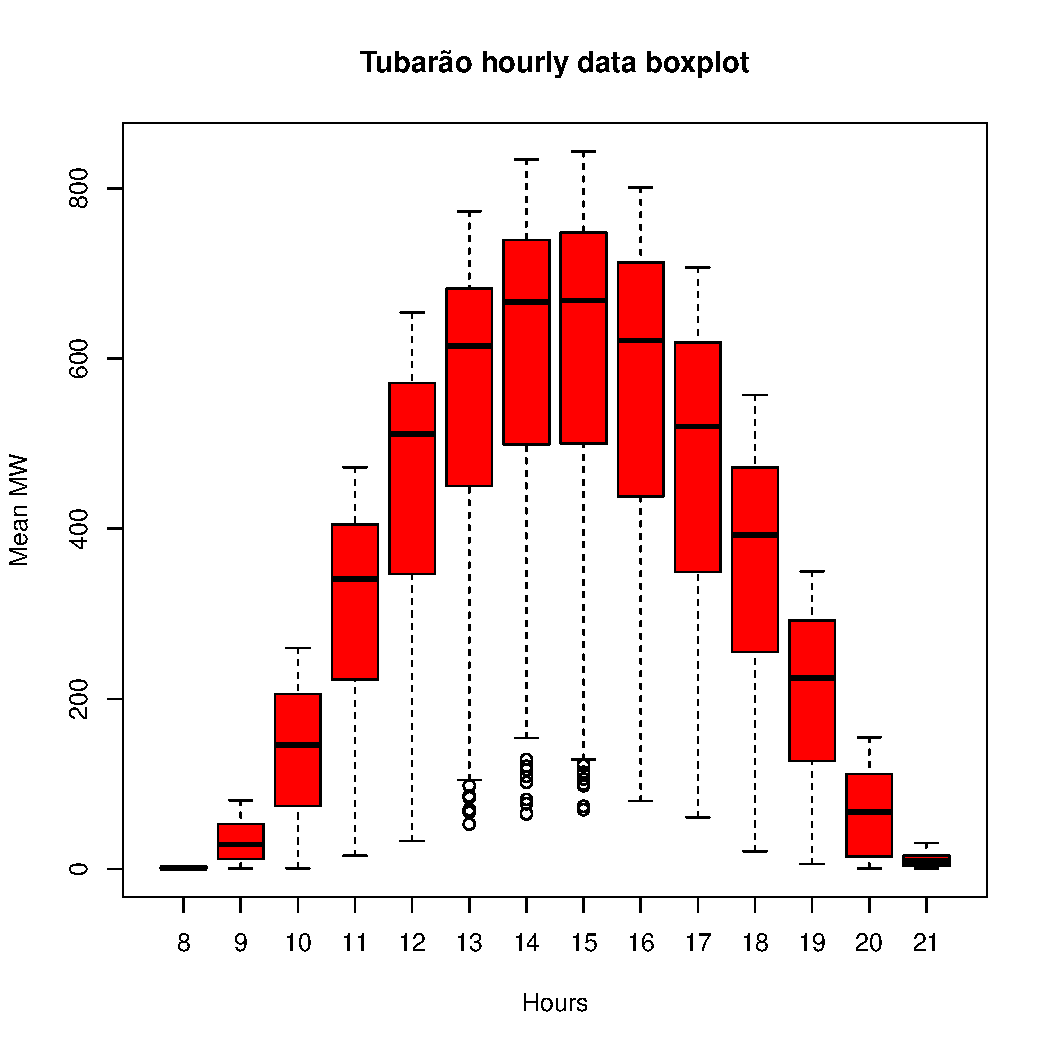
\includegraphics[width=\textwidth]{./../Figuras/Solar-exemplos/tubarao-boxplot}
%			%\caption{Boxplot for each month for the Icaraizinho dataset}
%			\label{fig:tubarao-boxplot}
%		\end{minipage}
%	\end{minipage}
%	\caption{Boxplots showing seasonality for monthly and hourly data.}
%	\label{fig:boxplots}
%\end{figure}



% % % % % % % % % % % % % PLANO DO ARTIGO % % % % % % % % % % % % % %


%1) Introdução
%
%2) Quantile Regression based time series model
%	A. Linear parametric explanatory model
%	B. General non-linear nonparametric model
%
%3) Estimation procedures
%	A. Linear model with optimal variable selection / regularization
%	B. Nonlinear model
%	
%4) Case study
%	A. Long term wind power generation
%	B. Short term wind (solar?) generation
%
%5) Conclusion










%\section*{Acknowledgment}

%The authors would like to thank FICO (Xpress-MP developer) for the academic partnership program with the Electrical Engineering Department of Pontifical Catholic University of Rio de Janeiro, Brazil (PUC-Rio). The authors would also like thank the LAMPS researchers for the daily exchanges and their insightful considerations.

%\IEEEtriggeratref{17}
\bibliographystyle{IEEEtran}
\bibliography{Thesis,QR,Bibhenriquinho}

%\begin{IEEEbiographynophoto}{Bruno Fanzeres} (S'11) has a B.Sc. degree in Electrical and Industrial Engineering and a M.Sc. degree in Operations Research from PUC-Rio, Brazil. He is pursuing a Ph.D degree in Operations Research at the same university.
%\end{IEEEbiographynophoto}

%\begin{IEEEbiographynophoto}{Arthur Brigatto} (S'14) received a B.Sc. degree in Electrical Engineering from the Federal University of Juiz de Fora, Brazil, and is pursuing a M.Sc. in Electrical Engineering at PUC-Rio, Brazil.
%\end{IEEEbiographynophoto}

%\begin{IEEEbiographynophoto}{Alexandre Street} (S'06, M'10) holds the degrees of M.Sc. and D.Sc. in Electrical Engineering (Operations Research) from PUC-Rio, Brazil. 
%\end{IEEEbiographynophoto}

%\begin{IEEEbiographynophoto}{Luiz Augusto Barroso} (S'00, M'06, SM'07) has a B.Sc. in Mathematics and a Ph.D degree in Operations Research. He is a technical director at PSR.
%\end{IEEEbiographynophoto}

\end{document}
